Padrão para enunciar uma fórmula




\begin{secnivel}{I}{Velocidade Vetorial Média}
  
  \eqLdois{def}{cinvet_eq_velocidadevetorialmedia}{\vec{v}_m := \dfrac{\Delta \vec{r}}{\Delta t}}

\end{secnivel}




\subsubsection{De onde vem}



\subsubsection{Onde é usada}



\subsubsection{Erros comuns}




\subsubsection{Observações}



\vspace{0.3cm}


\begin{exemplo}[Nível II]\label{exemplo_cinvet_velocidadeangularelinearex02}


\resolucao


\end{exemplo}

\vspace{0.3cm}





%Exemplo resolvido

\begin{tcolorbox}[enhanced,attach boxed title to top center={yshift=-3mm,yshifttext=-1mm},
  colback=gray!5!white,colframe=gray!75!black,colbacktitle=gray!80!black,
  title=Exemplo Resolvido,fonttitle=\bfseries,
  boxed title style={size=small,colframe=gray!50!gray} ]

Enuncie o exercício aqui.



\noindent\rule[0.5ex]{\linewidth}{1pt}

Resolva o exemplo aqui.

  
\end{tcolorbox}







Figura


\begin{figure}[h]
    \centering
    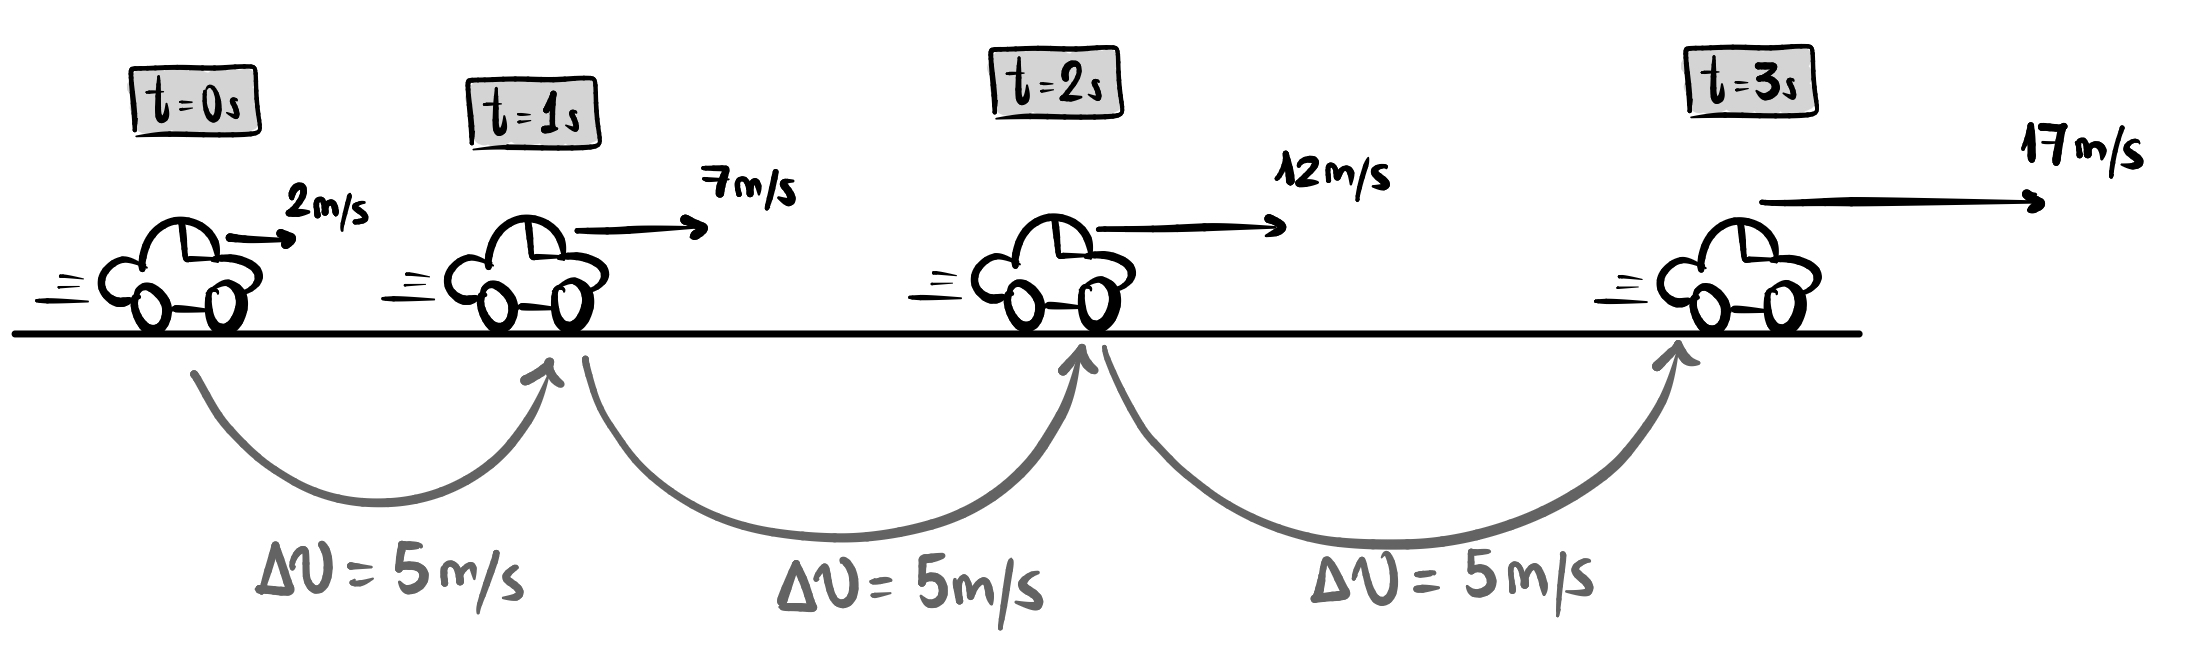
\includegraphics[scale=0.18]{imagensmecanica/acelerecao02.jpeg}
    \caption{Carro em movimento acelerado e o padrão de aumento de velocidade}
    \label{fig_mec_aceleracao02}
\end{figure}


\vspace{0.3cm}
{
\centering
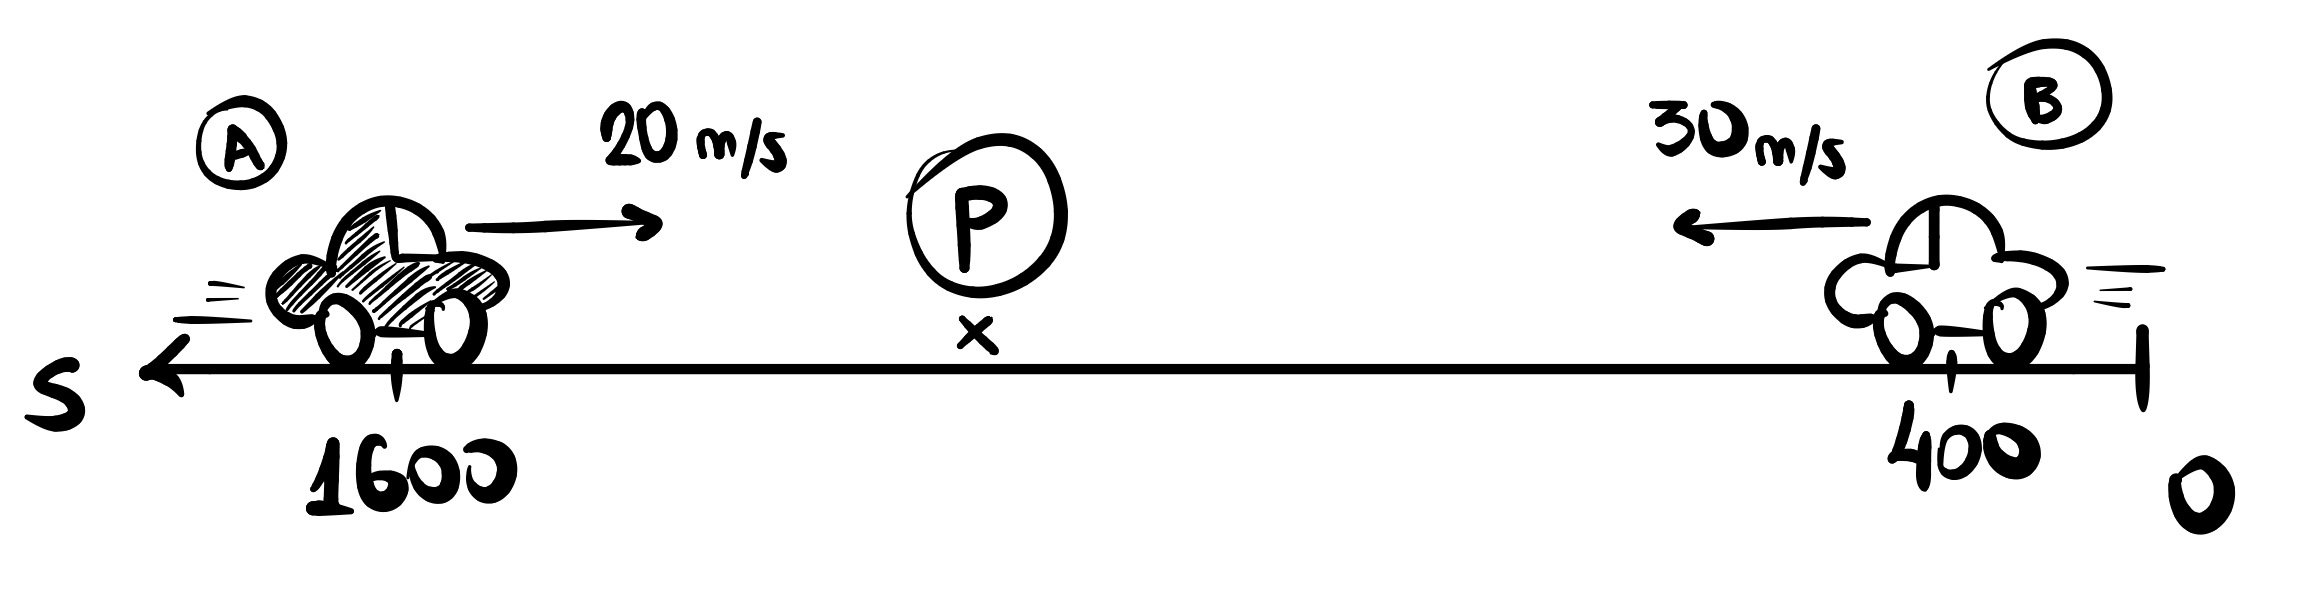
\includegraphics[width=0.6\linewidth]{imagensmecanica/sorveteexemplo013.jpeg}
\captionof{figure}{Referencial orientado para esquerda com origem arbitrária.}
\label{fig_mec_sorveteexemplo013}
} 
\vspace{0.3cm}




Apendices:


1 - área do gráfico vxt fornecer a distancia

2 - vetores

3 - 

4 - 

5 - 

Último - Equações demonstráveis vs experimentais (exemplo da lei de snell, que surge do experimento mas depois pode ser demonstrada por meio de um princípio postulado)

